\section{Curva A}

En esta punto se presenta una nueva herramienta gráfica que permite la evaluación de un modelo predictivo en base al error que se comente en la predicción. Este nuevo método surge de la necesidad de obtener una forma de representación gráfica que se pueda aplicar tanto a modelos de clasificación binaria como a modelos de clasificación multi etiqueta. La representación gráfica del error se obtiene a partir la formula de verificación propuesta por Brier en el articulo \textit{Verification of Forecasts Expressed in Terms of Probability} \cite{brie_1950}.

\bigbreak

La formula de verificación de Brier se define como el sumatorio del error cuadrático medio entre la clase y las diferentes probabilidades que asigna el modelo a cada etiqueta. La formula de verificación constituye un punto de partida ideal ya que se define teniendo en cuenta su aplicación a modelos de clasificación con mas de dos clases. La representación del error que se hace en la formula de verificación también es independiente del balance entre el numero de instancias de cada clase, esto supone un punto positivo a tener en cuenta.

\bigbreak

\begin{equation}
    P = \frac{1}{n}\sum_{j=1}^{r}\sum_{i=1}^{n}{(f_{ij}-E_{ij})^{2}}
    \label{eq:BrierScore}
\end{equation}

\bigbreak


En la ecuación \ref{eq:BrierScore} se representa la definición original de la formula de verificación. El parámetro $E_{ij}$ indica si la clase del registro $i$ coincide con la etiqueta $j$. El indicador $f_{ij}$ representa la probabilidad que se le asigna al registro $i$ de pertenecer a la clase $j$.

\bigbreak

El resultado que se obtiene al aplicar la formula de verificación se encuentra en el intervalo de cero a dos. En el caso de un modelo de clasificación binario en el que se predicen positivos los registros negativos y negativos los registros positivos, el resultado obtenido es de dos unidades. Por el contrario, si se clasifican correctamente todos los registros, el resultado obtenido es de cero.

\bigbreak

Para facilitar la interpretación de la curva A, se propone una modificación de la formula de verificación. El objetivo de redefinir la formula es obtener una gráfica que tenga una interpretación similar a la curva ROC. En la ecuación \ref{eq:A} aparece representada la formula que se utilizara en el calculo de la curva A. El resultado que se obtiene de la nueva formula se encuentra en el intervalo de cero a uno, los valores próximos a uno indican tasas de error mas bajas, mientras que los valores próximos a cero indican tasas de error mas altas. Hay que tener en cuenta que la aplicación del método ya no se hace sobre todas las instancias del modelo, si no que se aplica de forma individual a cada registro.

\bigbreak

\begin{equation}
    A = 1-\frac{\sum_{i=1}^{r}{(f_{i}-E_{i})^{2}}}{2}
    \label{eq:A}
\end{equation}

\bigbreak



La representación de la curva A se hace a partir del los valores obtenidos al aplicar la formula \ref{eq:A} a cada uno de los registros del conjunto de entrenamiento. Es importante aclarar que antes de generar la curva el conjunto de datos con los resultados tiene que estar ordenado. Para representar los puntos en la gráfica, a cada resultado se le asigna un valor equidistante entre cero y uno que permite representar los resultados obtenidos en base al orden establecido. En el eje de ordenadas se representan los resultados obtenidos al aplicar la formula, en el eje de abscisas se representan los puntos de apoyo calculados para cada resultado.

\bigbreak

La interpretación que se hace de la gráfica es muy similar a la que se hace en la curva ROC, cuanto mas se aproxime la gráfica al punto $(0, 1)$ mejores tasas de acierto tendrá el modelo. Las curvas que se encuentren por debajo de la diagonal secundaria indican que el modelo tiene tasas de acierto inferior a las de un modelo de clasificación aleatoria. En la Figura \ref{fig:1} se puede ver en azul la curva que presenta un modelo con una clasificación perfecta, por otro lado, la curva naranja es la curva que presenta un modelo de clasificación aleatoria.

\bigbreak

\begin{figure}[htp]
    \centering
    \includegraphics[scale=0.45]{interpretación_curva_a.PNG}
    \caption{Gráfica para la interpretación de la curva A.}
    \label{fig:1}
\end{figure}

\bigbreak

En la Figura \ref{fig:2} se muestra una comparativa entre las curvas A y ROC obtenidas para un modelo de clasificación con cuatro etiquetas. En el primer gráfico se puede observar que la aplicación de la curva ROC en un modelo con cuatro etiquetas implica un aumento de la complejidad en la interpretación de los resultados. El uso de curvas ROC en modelos de clasificación multi etiqueta, también afecta a las conclusiones que se pueden extraer de la calidad general del modelo, esta incapacidad de sacar conclusiones afecta negativamente al proceso de toma de decisiones. La curva A supone una excelente alternativa, el gráfico que se genera para un modelo de clasificación con cuatro etiquetas esta compuesto tan solo por una curva, esto supone una mejora en la claridad y en la interpretación de la información. 

\bigbreak

\begin{figure}[htp]
    \centering
     \subfloat[Curva ROC]{
       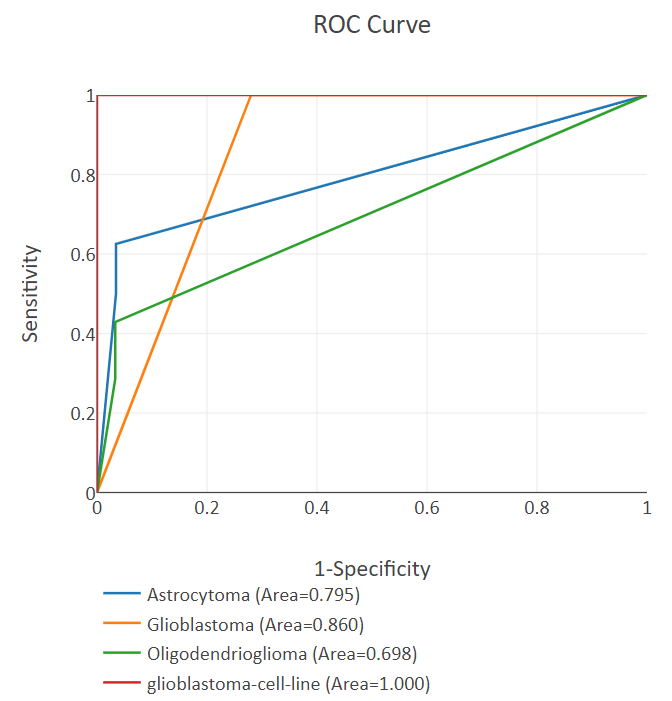
\includegraphics[width=0.45\textwidth]{brain_gse15824_ROC.PNG}}
     \subfloat[Curva A]{
       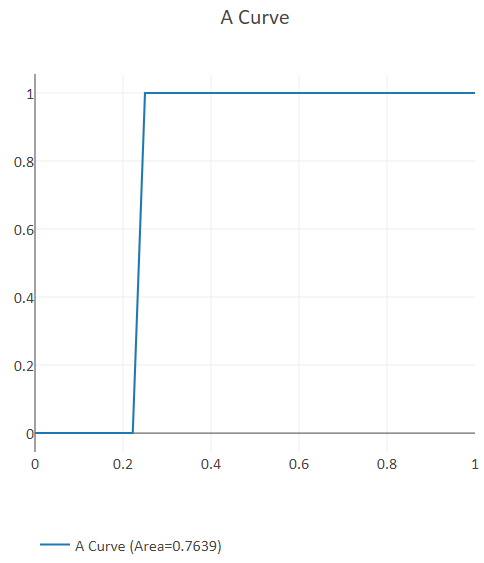
\includegraphics[width=0.45\textwidth]{brain_gse15824_A_CURVE.PNG}}
    \caption{Curvas obtenidas para el fichero brain\_gse15824.csv.}
    \label{fig:2}
\end{figure}

\bigbreak


Hay situaciones en las que no es posible establecer una comparativa exclusivamente gráfica entre varias representaciones de la curva A. La definición que se hace de la curva implica que el área bajo la curva aumenta a medida que la curva se aproxima al punto (0, 1), es decir, cuanto mayor es el valor de la área bajo la curva, mejores tasas de acierto obtiene el modelo. El área bajo la curva, también se puede considerar como un indicador de la calidad general del modelo. El resultado que ofrece, se encuentra en el intervalo de cero a uno, los valores cercanos a uno indican que el modelo tiene buenas tasas de acierto en la predicción, mientras que los valores próximos a cero indican la presencia de un modelo con una muy baja capacidad predictiva. Por último, cabe destacar el grado de similitud entre la exactitud y el área bajo la curva A, esta relección será objeto de estudio en la parte experimental.

\clearpage